% --- PREÁMBULO ---
% Aquí se definen el tipo de documento, los paquetes que usaremos, etc.
\documentclass[12pt, letterpaper]{article} % Tipo de documento

% --- PAQUETES ---
\usepackage[utf8]{inputenc} % Permite usar tildes y caracteres en español
\usepackage[spanish]{babel} % Configura el idioma español (para títulos, etc.)
\usepackage{geometry} % Para configurar márgenes
\usepackage{graphicx} % Para incluir imágenes
\usepackage{placeins} 

% Configuración de márgenes
\geometry{left=2.5cm, right=2.5cm, top=3cm, bottom=3cm}

% --- INFORMACIÓN DEL DOCUMENTO ---
\title{Extensión para Visual Studio Code como simulador para procesador RISC-V}
\author{Amir Evelio Hurtado Mena \\ \texttt{a.hurtado@utp.edu.co}}
\date{\today} % Pone la fecha de hoy, puedes cambiarla si quieres


% --- COMIENZO DEL DOCUMENTO ---
\begin{document}

\begin{titlepage}
    \centering % Centra todo el contenido de la página

    % Encabezado de la universidad
    \textsc{\LARGE UNIVERSIDAD TECNOLÓGICA DE PEREIRA} \\[0.5cm]
    \textsc{\Large FACULTAD DE INGENIERÍAS} \\[0.5cm]
    \textsc{\large Programa de Ingeniería de Sistemas y Computación} \\[2cm]

    % Título del trabajo
    \rule{\textwidth}{0.4pt}\\[0.4cm]
    { \huge \bfseries Extensión para Visual Studio Code como simulador para procesador RISC-V \\[0.4cm] }
    \rule{\textwidth}{0.4pt}\\[2cm]

    % Información del estudiante
    \begin{flushleft} % Alinea el siguiente bloque a la izquierda
    \textbf{Autor:} \\
    Amir Evelio Hurtado Mena \\
    \textbf{Código:} 1077997025 \\
    \textbf{Email:} a.hurtado@utp.edu.co \\[1cm]

    \textbf{Director:} \\
    % Aquí pones el nombre de tu director cuando lo tengas
    (Nombre del Director) \\[2cm]
    \end{flushleft}

    % Información del proyecto
    \begin{center} % Centra este bloque específico
    \textbf{Área Temática:} Ingeniería de Software \\
    \textbf{Línea de Investigación:} Desarrollo de Software Aplicado  \\[0.5cm]
    \textbf{Modalidad:} Proyecto de Aplicación  \\[2cm]
    \end{center}

    \vfill % Empuja el contenido siguiente hacia el final de la página

    % Fecha
    Pereira, Colombia \\
    \today

\end{titlepage}

\newpage % Crea una nueva página para empezar el contenido

\tableofcontents % Crea el índice






% --- INTRODUCCIÓN ---
\newpage 
\section{Introducción}

La Arquitectura de Computadores es una materia fundamental en la carrera de Ingeniería de Sistemas y Computación, ya que permite entender cómo funciona el hardware que ejecuta todo el software que creamos. Sin embargo, los conceptos sobre el funcionamiento interno de un procesador, como los registros, las unidades de control y los ciclos de instrucción, suelen ser muy abstractos y dificiles de asimilar para los estudiantes que cursan la asignatura en la Universidad Tecnológica de Pereira.

Esta dificultad a menudo genera un obstáculo en el proceso de aprendizaje, ralentizando el avance de las clases y dejando vacíos conceptuales en los futuros profesionales. Para abordar este problema, este proyecto propone el desarrollo de una herramienta de software: una extensión para el editor de código Visual Studio Code que funciona como un simulador gráfico e interactivo de un procesador con arquitectura RISC-V, tanto en su versión monociclo como segmentada.

El objetivo es ofrecer a estudiantes y docentes un recurso que traduzca las operaciones complejas del procesador en visualizaciones claras y fáciles de seguir. De esta manera, se busca fortalecer la comprensión de los temas clave de la materia, haciendo el aprendizaje más práctico, intuitivo y efectivo, y mejorando así la calidad de la formación de los ingenieros de la universidad.




% --- PLANTEAMIENTO DEL PROBLEMA ---
\section{Planteamiento del problema}

% --- Subsección de Antecedentes---
\subsection{Antecedentes (Contextualización del problema)}
La enseñanza de la Arquitectura de Computadores presenta desafios pedagógicos bien documentados en la literatura académica... (el resto del texto de antecedentes va aquí, sin cambios) ...para mejorar significativamente la experiencia educativa en esta área fundamental.

% --- Subsección de Causas  ---
\subsection{Causas (qué está causando el problema)}
La causa principal del problema en la asignatura de Arquitectura de Computadores de la UTP es la brecha existente entre la teoría abstracta enseñada en clase y la falta de herramientas prácticas que permitan a los estudiantes visualizar y experimentar con dichos conceptos. Esta situación fue validada a través de una encuesta realizada a 57 estudiantes del programa que ya habían cursado la materia. Los resultados revelan la magnitud del desafío: un contundente 86\% de los estudiantes calificó el proceso de comprensión de la arquitectura de un computador y su implementación en hardware como "Complejo" o "Muy complejo", lo que demuestra que no se trata de una percepción aislada, sino de una dificultad generalizada en el alumnado (Ver Gráfico \ref{fig:grafico1}).

\begin{figure}[h!]
    \centering
    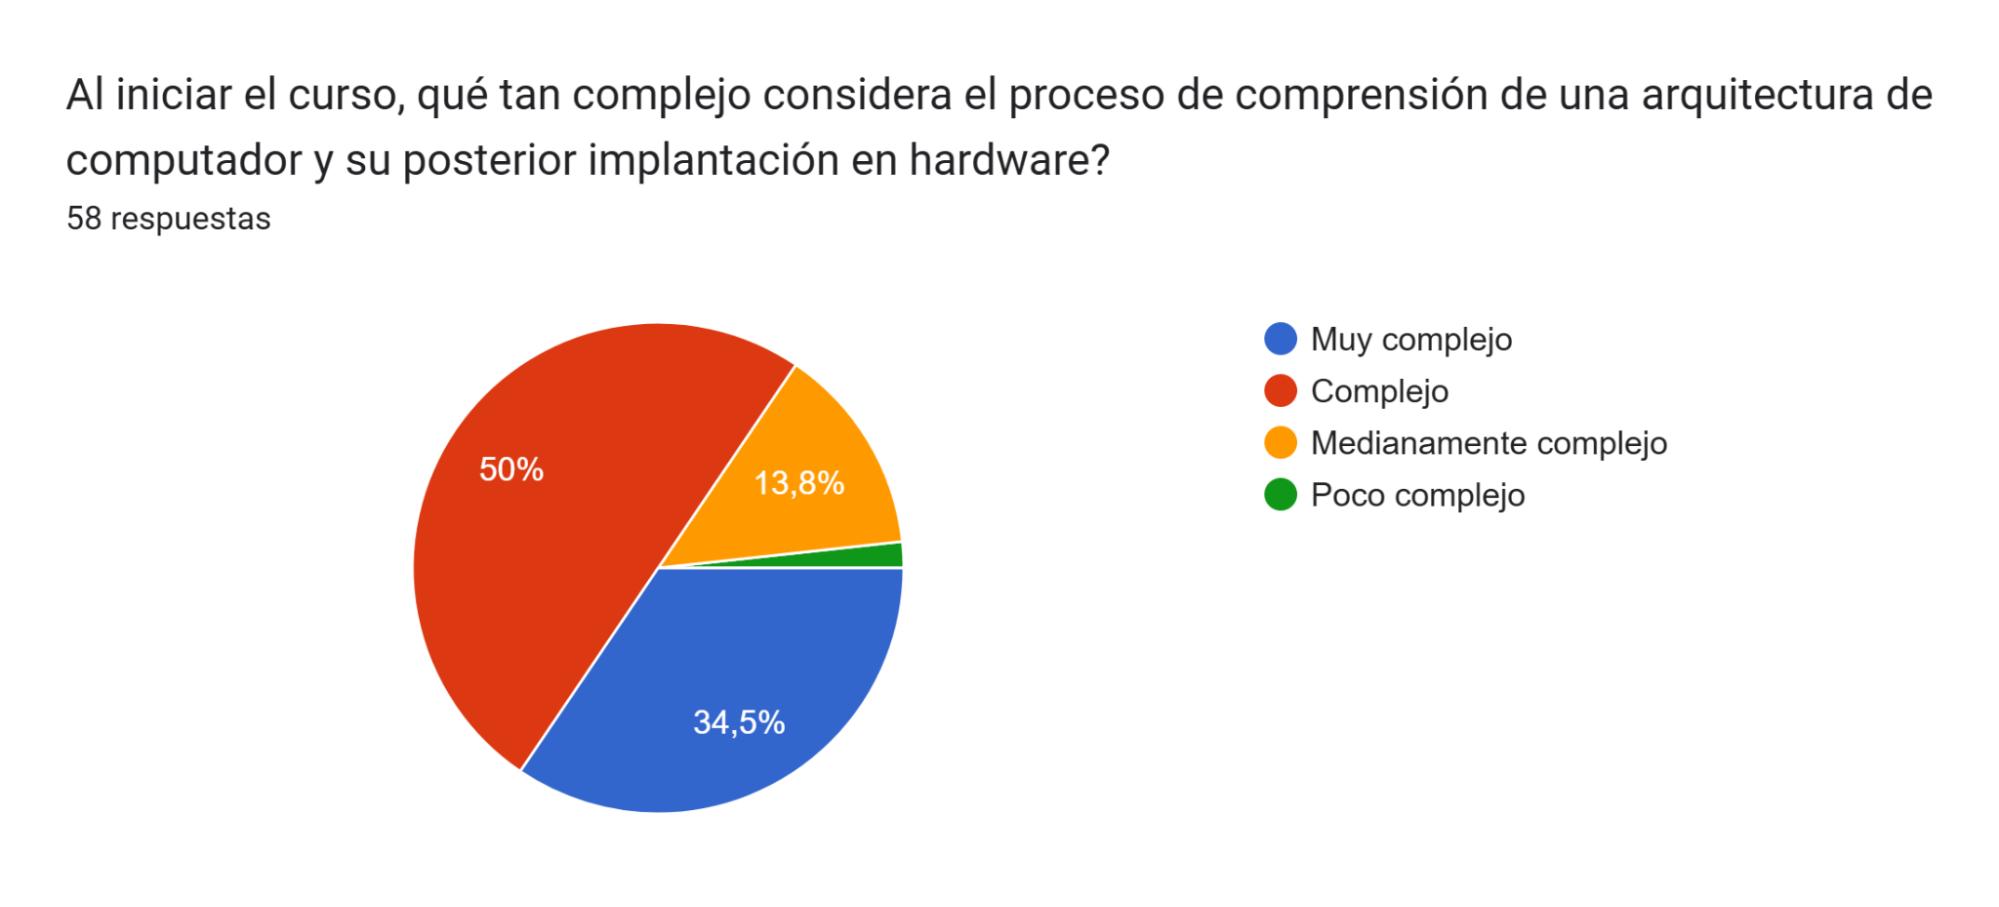
\includegraphics[width=0.7\textwidth]{figura1.png}
    \caption{Resultados sobre la complejidad percibida.}
    \label{fig:grafico1}
\end{figure}


\FloatBarrier %

Más importante aún, la encuesta también indagó sobre la solución a esta dificultad. Al preguntarles sobre la necesidad de una nueva herramienta, la respuesta fue abrumadora: un 91.1\% de los estudiantes (sumando las categorías "Muy necesario" y "Necesario") afirmó que la inclusión de una herramienta tecnológica para visualizar los conceptos sería clave para un mejor aprendizaje (Ver Gráfico \ref{fig:grafico2}).  Estos datos demuestran que la causa del problema no es una falta de interés por parte del alumnado, sino una necesidad directa y explícita de un recurso didáctico interactivo que les permita conectar los conceptos abstractos con una representación visual y práctica. La herramienta propuesta en este proyecto busca, por lo tanto, atacar directamente esta causa raíz.

\begin{figure}[h!]
    \centering
    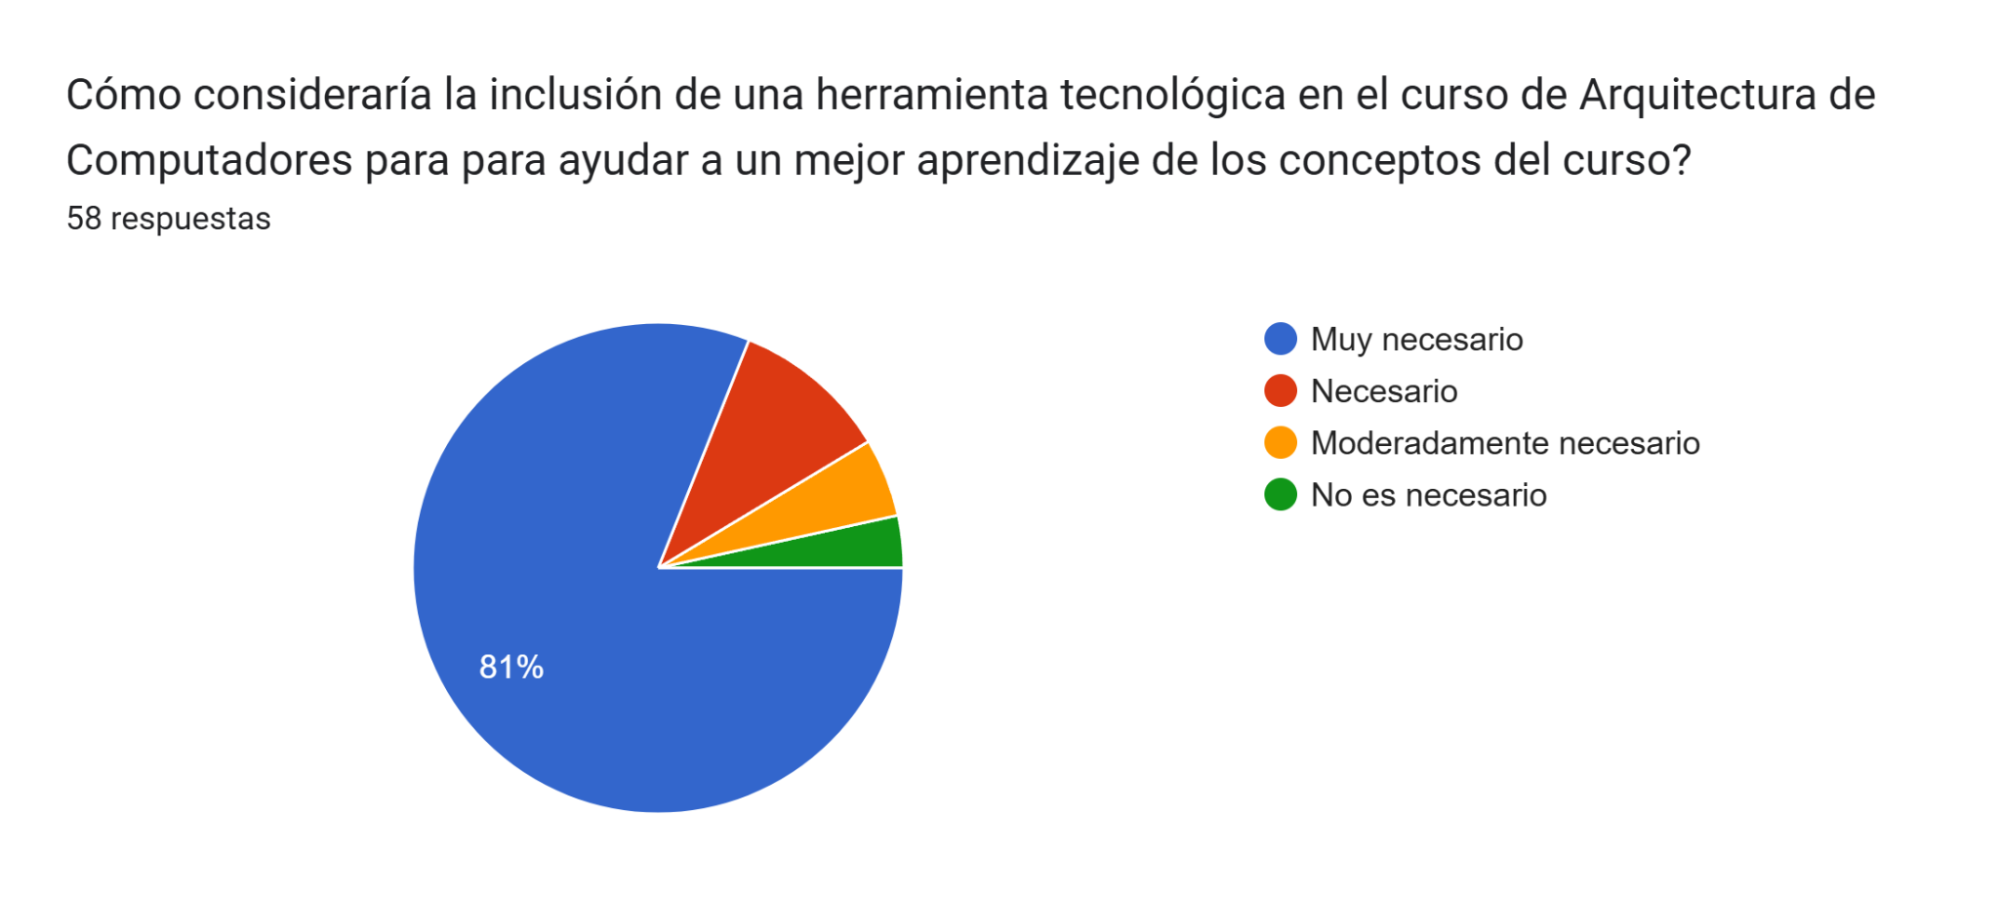
\includegraphics[width=0.8\textwidth]{figura2.png}
    \caption{Necesidad de una herramienta tecnológica según los estudiantes.}
    \label{fig:grafico2}
\end{figure}

% --- Subsección de Definición del Problema ---
\subsection{Definición del problema}
Los estudiantes de la asignatura de Arquitectura de Computadores del programa de Ingeniería de Sistemas y Computación de la UTP presentan dificultades significativas para comprender los procesos internos de un procesador (monociclo y segmentado).

% --- Subsección de Consecuencias ---
\subsection{Consecuencias (de no resolver el problema)}
De no abordarse este problema, las consecuencias afectan a múltiples niveles. Para los estudiantes, implica una base conceptual débil que puede perjudicar su desempeño en materias posteriores que dependen de estos conocimientos, además de generar frustración y desinterés por el área del hardware. Para los docentes, significa tener que invertir más tiempo en reforzar conceptos básicos, ralentizando el avance del temario y limitando la posibilidad de profundizar en temas más avanzados. A largo plazo, para el programa académico, esto representa un riesgo en la calidad de la formación, ya que sus egresados podrían tener vacíos en un área fundamental de la ingeniería de sistemas, lo que podría impactar negativamente su perfil profesional en el mercado laboral.







\end{document}





